\documentclass{article}
\usepackage{sagetex}
\usepackage{tikz,tkz-graph,tkz-berge}
\thispagestyle{empty}
\begin{document}
Here's a graph where you specify the position of the vertices. Note that  the label is placed inside unless specified:\\\\
\begin{center}
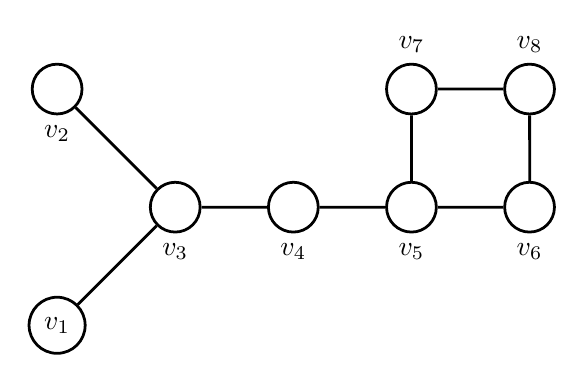
\begin{tikzpicture}[scale=1.5]
\renewcommand*{\VertexLineWidth}{1pt}%vertex thickness
\renewcommand*{\EdgeLineWidth}{1pt}% edge thickness
\GraphInit[vstyle=Normal]
\Vertex[Lpos=270,L=$v_1$,x=0,y=0]{R1}
\Vertex[LabelOut,Lpos=270,L=$v_2$,x=0,y=2]{R2}
\Vertex[LabelOut,Lpos=270,L=$v_3$,x=1,y=1]{R3}
\Vertex[LabelOut,Lpos=270,L=$v_4$,x=2,y=1]{R4}
\Vertex[LabelOut,Lpos=270,L=$v_5$,x=3,y=1]{R5}
\Vertex[LabelOut,Lpos=270,L=$v_6$,x=4,y=1]{R6}
\Vertex[LabelOut,Lpos=90,L=$v_7$,x=3,y=2]{R7}
\Vertex[LabelOut,Lpos=90,L=$v_8$,x=4,y=2]{R8}
%%%%%%%%%%%%%%%%%%%%%%%%%%%%%%
\Edge (R3)(R4)
\Edge (R3)(R1)
\Edge (R2)(R3)
\Edge (R5)(R4)
\Edge (R5)(R6)
\Edge (R5)(R7)
\Edge (R6)(R8)
\Edge (R7)(R8)
\end{tikzpicture}
\end{center}

But \textsf{Sage} has knowledge of graph theory and you can use it to specify graphs
and determine various characteristics. For example:\\\\
\begin{sagesilent}
H= graphs.PetersenGraph()
H.set_latex_options(scale=3.5,graphic_size=(2.1,2.1))
Chi = H.chromatic_number(algorithm="DLX")
Beta = H.independent_set()
\end{sagesilent}
\noindent The Petersen graph below has $\sage{H.order()}$ vertices and
$\sage{H.size()}$ edges.\\\\
\begin{center}
\begin{tikzpicture}
\GraphInit[vstyle=Normal]
\SetVertexNormal[Shape=circle,LineWidth = 1pt]
\tikzset{EdgeStyle/.append style = {color = blue!60, line width=1pt}}
\sage{H}
\end{tikzpicture}
\end{center}
\vspace{5pt}
The chromatic number is $\chi(G)=\sage{Chi}$. The maximum size independent 
set is $\beta(G)=\sage{len(Beta)}$. One such set is $\sage{Beta}$. The 
maximum size clique has $\omega(G)=\sage{H.clique_number()}$ vertices; 
e.g., $\sage{H.clique_maximum()}$. The diameter is $\sage{H.diameter()}$
and the radius is $\sage{H.radius()}$.
\end{document}

